%% LyX 2.2.2 created this file.  For more info, see http://www.lyx.org/.
%% Do not edit unless you really know what you are doing.
\documentclass[english]{beamer}
\usepackage{mathptmx}
\usepackage{eulervm}
\usepackage[T1]{fontenc}
\usepackage[latin9]{inputenc}
\usepackage{amsmath}
\usepackage{amssymb}
\usepackage{graphicx}

\makeatletter

%%%%%%%%%%%%%%%%%%%%%%%%%%%%%% LyX specific LaTeX commands.
%% A simple dot to overcome graphicx limitations
\newcommand{\lyxdot}{.}


%%%%%%%%%%%%%%%%%%%%%%%%%%%%%% Textclass specific LaTeX commands.
 % this default might be overridden by plain title style
 \newcommand\makebeamertitle{\frame{\maketitle}}%
 % (ERT) argument for the TOC
 \AtBeginDocument{%
   \let\origtableofcontents=\tableofcontents
   \def\tableofcontents{\@ifnextchar[{\origtableofcontents}{\gobbletableofcontents}}
   \def\gobbletableofcontents#1{\origtableofcontents}
 }

%%%%%%%%%%%%%%%%%%%%%%%%%%%%%% User specified LaTeX commands.
\usetheme{CambridgeUS} 
\beamertemplatenavigationsymbolsempty

\AtBeginSection[]{
  \begin{frame}
  \vfill
  \centering
  \begin{beamercolorbox}[sep=8pt,center,shadow=true,rounded=true]{title}
    \usebeamerfont{title}\insertsectionhead\par%
  \end{beamercolorbox}
  \vfill
  \end{frame}
}

\makeatother

\usepackage{babel}
\begin{document}

\global\long\def\reals{\mathbf{R}}
\global\long\def\RR{\mathbf{R}}
 \global\long\def\integers{\mathbf{Z}}
 \global\long\def\naturals{\mathbf{N}}
 \global\long\def\rationals{\mathbf{Q}}
 \global\long\def\ca{\mathcal{A}}
 \global\long\def\cb{\mathcal{B}}
 \global\long\def\cc{\mathcal{C}}
 \global\long\def\cd{\mathcal{D}}
 \global\long\def\ce{\mathcal{E}}
 \global\long\def\cf{\mathcal{F}}
 \global\long\def\cg{\mathcal{G}}
 \global\long\def\ch{\mathcal{H}}
 \global\long\def\ci{\mathcal{I}}
 \global\long\def\cj{\mathcal{J}}
 \global\long\def\ck{\mathcal{K}}
 \global\long\def\cl{\mathcal{L}}
 \global\long\def\cm{\mathcal{M}}
 \global\long\def\cn{\mathcal{N}}
 \global\long\def\co{\mathcal{O}}
 \global\long\def\cp{\mathcal{P}}
 \global\long\def\cq{\mathcal{Q}}
 \global\long\def\calr{\mathcal{R}}
 \global\long\def\cs{\mathcal{S}}
 \global\long\def\ct{\mathcal{T}}
 \global\long\def\cu{\mathcal{U}}
 \global\long\def\cv{\mathcal{V}}
 \global\long\def\cw{\mathcal{W}}
 \global\long\def\cx{\mathcal{X}}
 \global\long\def\cy{\mathcal{Y}}
 \global\long\def\cz{\mathcal{Z}}
 \global\long\def\ind#1{1(#1)}
 %\newcommand{\pr}{P}
\global\long\def\pr{\mathbb{P}}
 \global\long\def\predsp{\cy}
 %{\hat{\cy}}
\global\long\def\outsp{\cy}

\global\long\def\prxy{P_{\cx\times\cy}}
 \global\long\def\prx{P_{\cx}}
 \global\long\def\prygivenx{P_{\cy\mid\cx}}
 %\newcommand{\ex}{E}
\global\long\def\ex{\mathbb{E}}
 \global\long\def\var{\textrm{Var}}
 \global\long\def\Ind{\mathbf{1}}
 \global\long\def\cov{\textrm{Cov}}
 \global\long\def\sgn{\textrm{sgn}}
 \global\long\def\sign{\textrm{sign}}
 \global\long\def\kl{\textrm{KL}}
 \global\long\def\law{\mathcal{L}}
 \global\long\def\eps{\varepsilon}
 \global\long\def\as{\textrm{ a.s.}}
 \global\long\def\io{\textrm{ i.o.}}
 \global\long\def\ev{\textrm{ ev.}}
 \global\long\def\convd{\stackrel{d}{\to}}
 \global\long\def\eqd{\stackrel{d}{=}}
 \global\long\def\del{\nabla}
 \global\long\def\loss{\ell}
 \global\long\def\risk{R}
 \global\long\def\emprisk{\hat{R}}
 \global\long\def\lossfnl{L}
 \global\long\def\emplossfnl{\hat{L}}
 \global\long\def\empminimizer#1{\hat{#1}^{*}}
 \global\long\def\minimizer#1{#1^{*}}
\global\long\def\optimizer#1{#1^{*}}
 \global\long\def\etal{\textrm{et. al.}}
 \global\long\def\tr{\operatorname{tr}}

\global\long\def\trace{\operatorname{trace}}
 \global\long\def\diag{\text{diag}}
 \global\long\def\rank{\text{rank}}
 \global\long\def\linspan{\text{span}}
 \global\long\def\spn{\text{span}}
 \global\long\def\proj{\text{Proj}}
 \global\long\def\argmax{\operatornamewithlimits{arg\, max}}
 \global\long\def\argmin{\operatornamewithlimits{arg\, min}}

\global\long\def\bfx{\mathbf{x}}
 \global\long\def\bfy{\mathbf{y}}
 \global\long\def\bfl{\mathbf{\lambda}}
 \global\long\def\bfm{\mathbf{\mu}}
 \global\long\def\calL{\mathcal{L}}

\global\long\def\vw{\boldsymbol{w}}
 \global\long\def\vx{\boldsymbol{x}}
 \global\long\def\vxi{\boldsymbol{\xi}}
 \global\long\def\valpha{\boldsymbol{\alpha}}
 \global\long\def\vbeta{\boldsymbol{\beta}}
 \global\long\def\vsigma{\boldsymbol{\sigma}}
\global\long\def\vtheta{\boldsymbol{\theta}}
 \global\long\def\vd{\boldsymbol{d}}
 \global\long\def\vs{\boldsymbol{s}}
 \global\long\def\vt{\boldsymbol{t}}
 \global\long\def\vh{\boldsymbol{h}}
 \global\long\def\ve{\boldsymbol{e}}
 \global\long\def\vf{\boldsymbol{f}}
 \global\long\def\vg{\boldsymbol{g}}
 \global\long\def\vz{\boldsymbol{z}}
 \global\long\def\vk{\boldsymbol{k}}
 \global\long\def\va{\boldsymbol{a}}
 \global\long\def\vb{\boldsymbol{b}}
 \global\long\def\vv{\boldsymbol{v}}
 \global\long\def\vy{\boldsymbol{y}}

\global\long\def\hil{\ch}
 \global\long\def\rkhs{\hil}
 \global\long\def\ber{\text{Ber}}


\title[DS-GA 1003 ]{Gaussian Mixture Models}

\author{David Rosenberg, Brett Bernstein}

\date{\today}

\institute{New York University}

\makebeamertitle

\section{Intro Question}
\begin{frame}{Intro Question}
  Suppose we begin with a dataset $\cd = \{x_1,\ldots,x_n\}\subseteq\RR^2$
  and we run $k$-means (or $k$-means$++$) to obtain $k$ cluster
  centers.  Below we have drawn the cluster centers.  If we are given
  a new $x\in\RR^2$, we can assign it a label based on which cluster
  center is closest.  What regions of the plane below correspond to
  each possible labeling?
\end{frame}
\begin{frame}{Intro SOlution}
  \begin{itemize}
  \item Note that each cell is disjoint (except for the boarders), and
    convex.
  \item This can be thought of as a limitation of $k$-means.
  \end{itemize}
\end{frame}
\section{Gaussian Mixture Models}
\begin{frame}{Yesterday's Intro Question}
  Consider the following probability model for generating data.
  \begin{enumerate}
  \item Roll a weighted $k$-sided die to choose a label
    $z\in\{1,\ldots,k\}$.  Let $\pi$ denote the PMF for the die.
  \item Draw $x\in\reals^d$ randomly from the multivariate normal
    distribution $\cn(\mu_z,\Sigma_z)$.
  \end{enumerate}
  Solve the following questions.
  \begin{enumerate}
  \item What is the joint distribution of $x,z$ given $\pi$ and the
    $\mu_z,\Sigma_z$ values?
  \item Suppose you were given the dataset
    $\cd=\{(x_1,z_1),\ldots,(x_n,z_n)\}$.  How would you estimate the
    die weightings, and the $\mu_z,\Sigma_z$ values?
  \item How would you determine the label for a new datapoint $x$?
  \end{enumerate}
\end{frame}
\begin{frame}{Yesterday's Intro Solution}
  \begin{enumerate}
  \item The joint PDF/PMF is given by
    $$p(x,z) = \pi(z)f(x;\mu_z,\Sigma_z)$$
    where
    $$f(x;\mu_z,\Sigma_z) =
    \frac{1}{\sqrt{|2\pi\Sigma_z|}}\exp\left(-\frac{1}{2}(x-\mu)^T\Sigma^{-1}(x-\mu)\right).$$
  \item We could use maximum likelihood estimation.  Our estimates are
    $$\begin{array}{rcl}
    n_z  & = & \sum_{i=1}^n \Ind(z_i=z) \\
    \hat{\pi}(z) & = & \frac{n_z}{n}\\
    \hat{\mu}_z & = & \frac{1}{n_z}\sum_{i:z_i=z} x_i\\
    \hat{\Sigma}_z & = & \frac{1}{n_z}\sum_{i:z_i=z} (x_i-\hat{\mu}_z)(x_i-\hat{\mu}_z)^T.
    \end{array}$$
  \item $\argmax_z p(x,z)$
  \end{enumerate}
\end{frame}
\begin{frame}{Probabilistic Model for Clustering}

\begin{itemize}
\item Let's consider a \textbf{generative model} for the data.
\item Suppose 

\begin{enumerate}
\item There are $k$ clusters.
\item We have a probability density for each cluster.
\end{enumerate}
\item Generate a point as follows

\begin{enumerate}
\item Choose a random cluster $z\in\left\{ 1,2,\ldots,k\right\} $. 
\item Choose a point from the distribution for cluster $Z$. 
\end{enumerate}
\item To find our clusters
\end{itemize}
\end{frame}

\begin{frame}{Gaussian Mixture Model ($k=3$)}

\begin{enumerate}
\item Choose $z\in\left\{ 1,2,3\right\} $ with $p(1)=p(2)=p(3)=\frac{1}{3}$. 
\item Choose $x\mid z\sim\cn\left(X\mid\mu_{z},\Sigma_{z}\right)$.
\end{enumerate}
\begin{center}
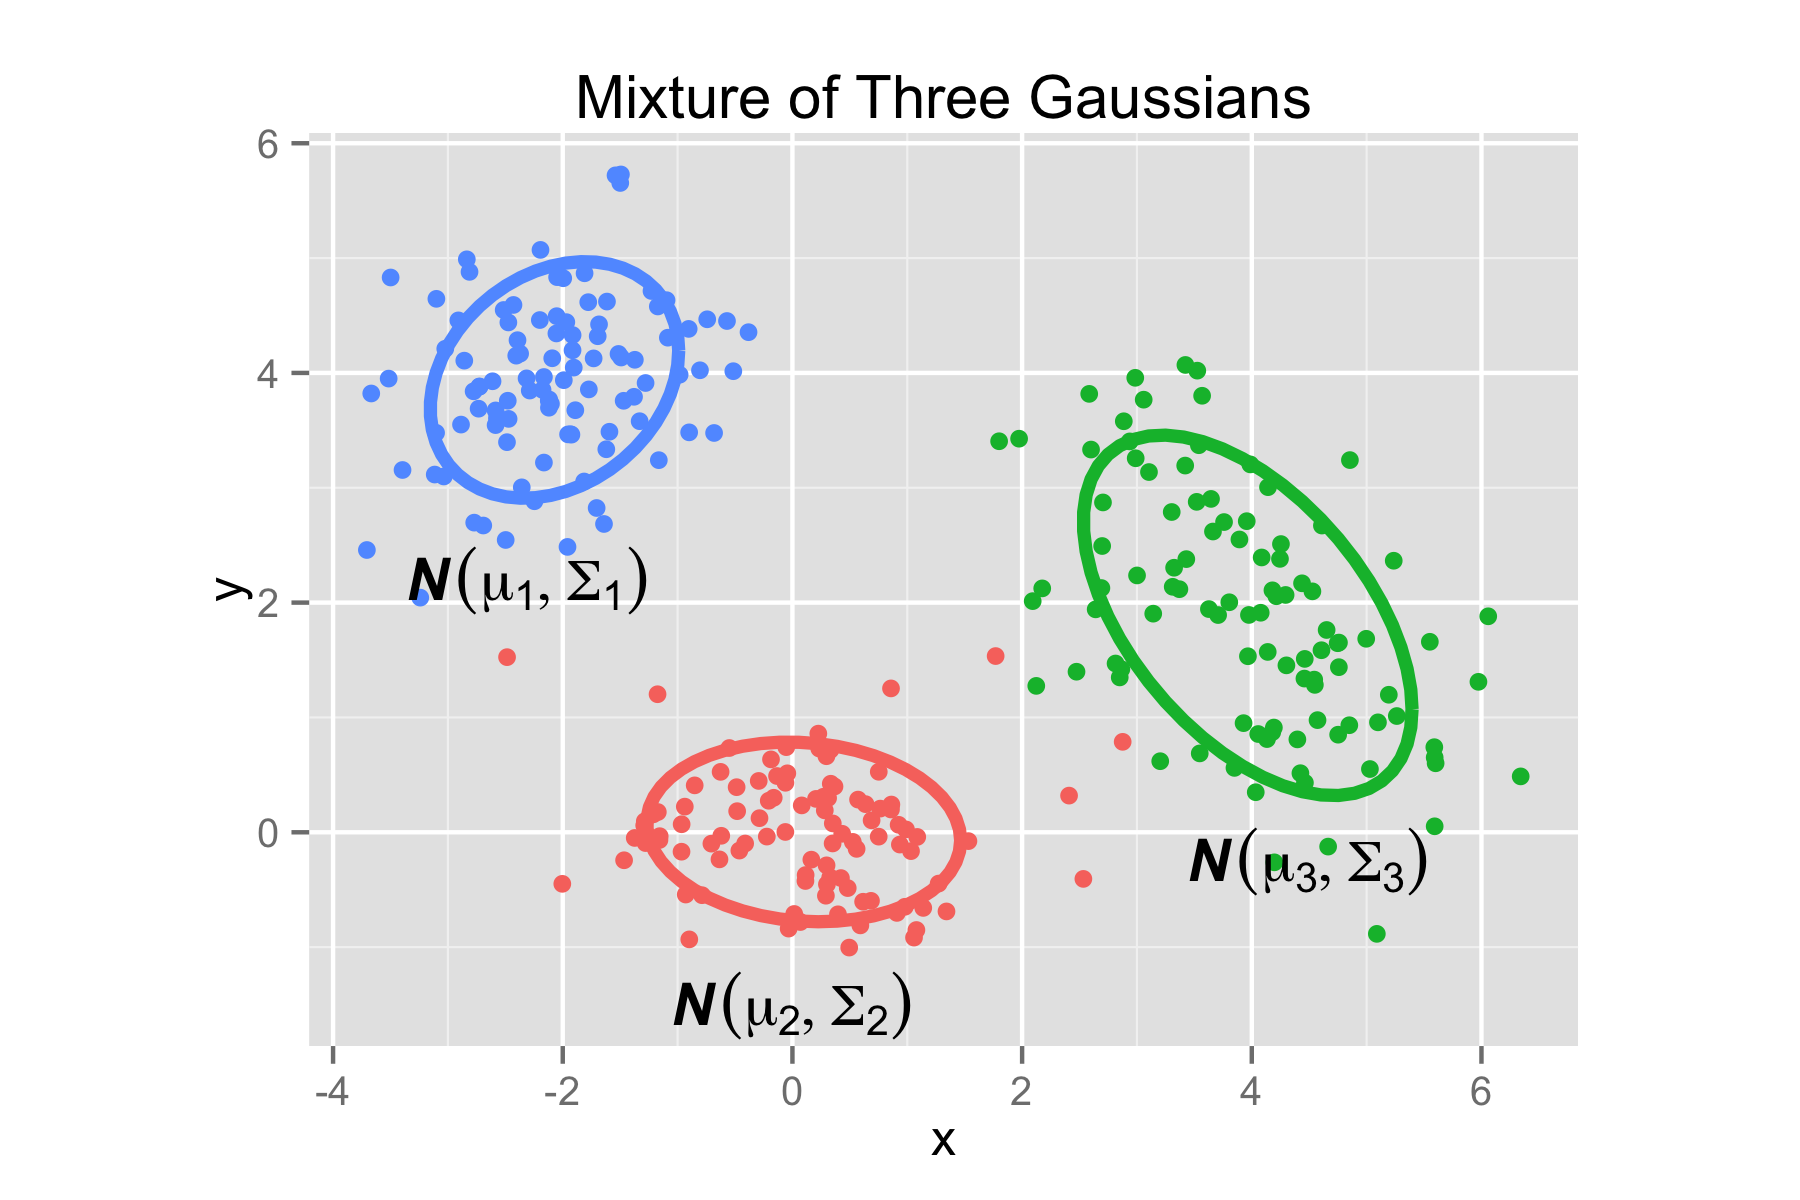
\includegraphics[width=0.7\textwidth]{../Figures/clustering/mixture-3-gaussians}
\par\end{center}

\end{frame}

\begin{frame}{Gaussian Mixture Model Parameters ($k$ Components)}

\begin{center}
\begin{eqnarray*}
\text{Cluster probabilities}: &  & \pi=\left(\pi_{1},\ldots,\pi_{k}\right)\\
\text{Cluster means}: &  & \mu=\left(\mu_{1},\ldots,\mu_{k}\right)\\
\text{Cluster covariance matrices:} &  & \Sigma=\left(\Sigma_{1},\ldots\Sigma_{k}\right)
\end{eqnarray*}
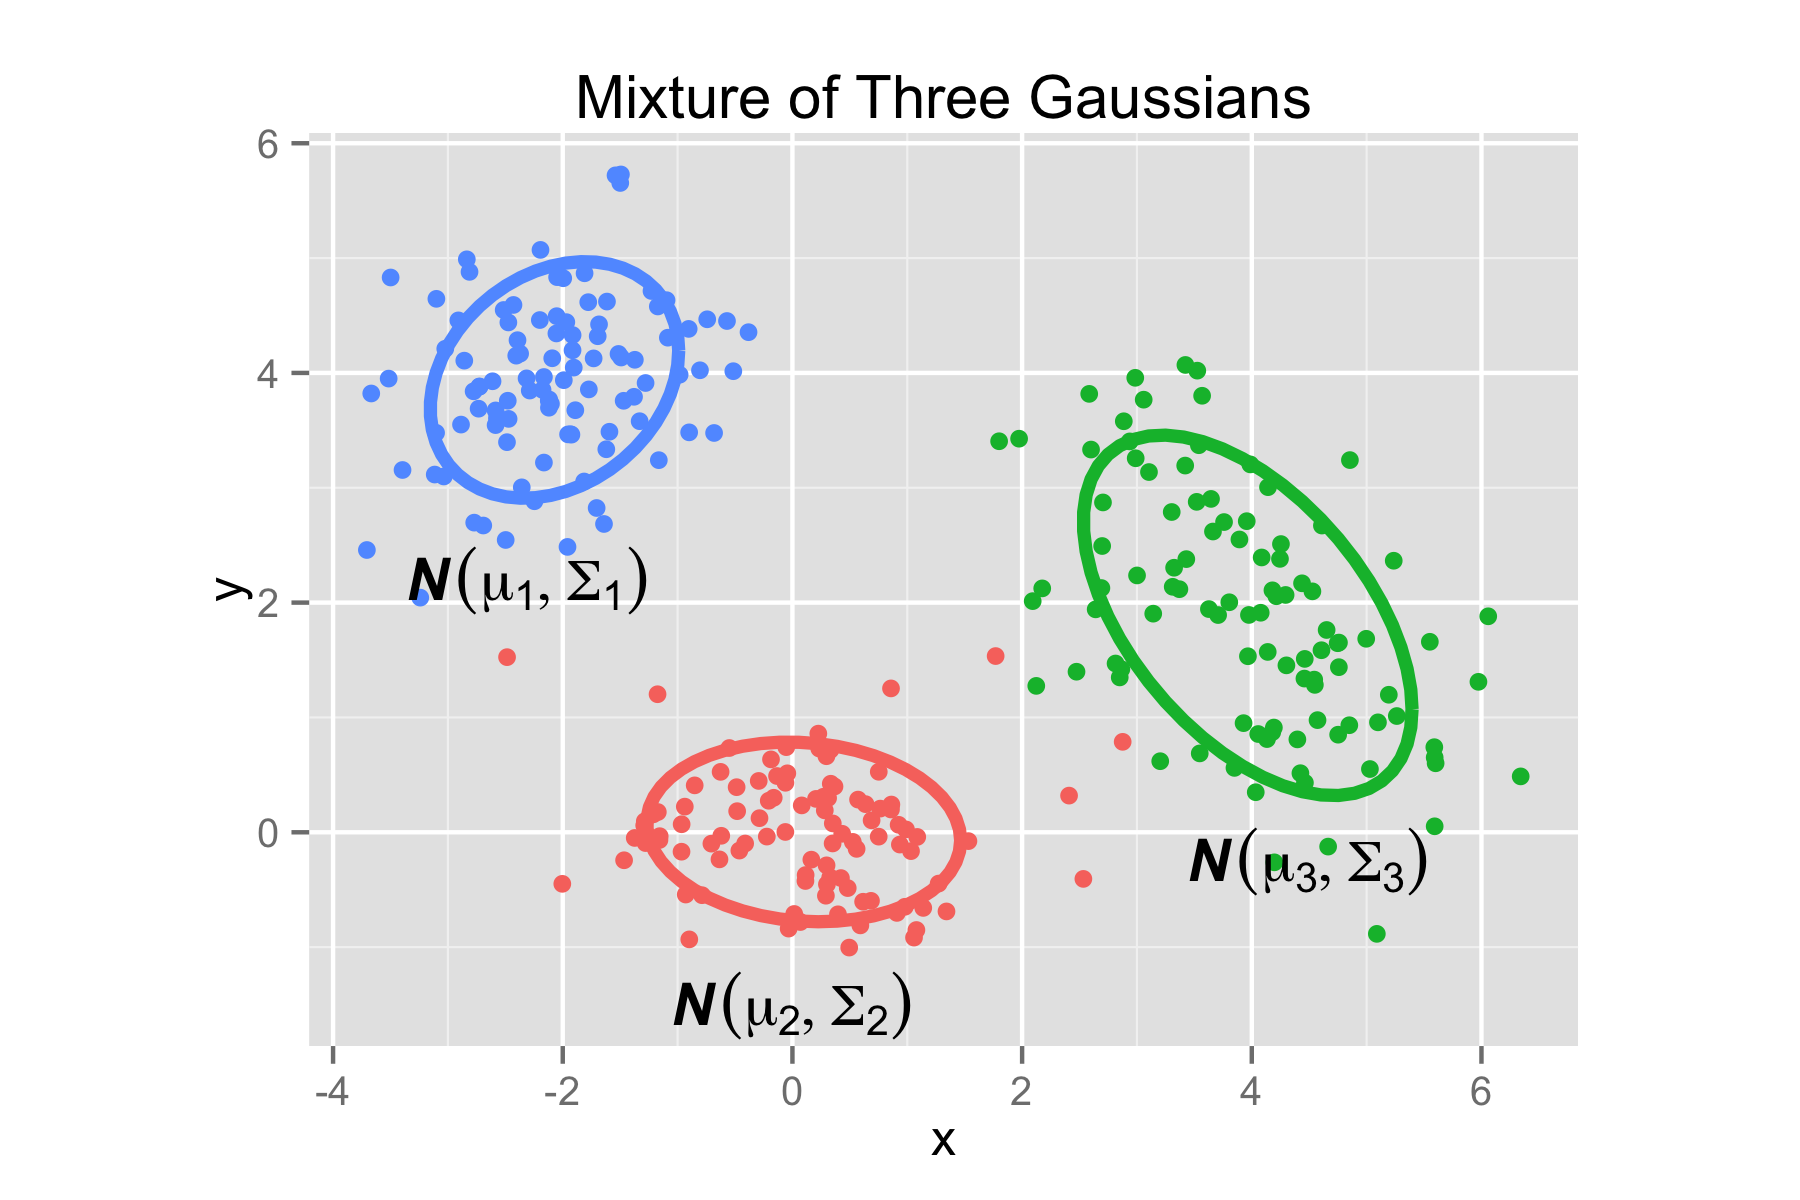
\includegraphics[height=0.4\textheight]{../Figures/clustering/mixture-3-gaussians} 
\par\end{center}


For now, \textbf{suppose all these parameters are known}. \\
We'll discuss how to \textbf{learn} or \textbf{estimate }them later.
\end{frame}

\begin{frame}{Gaussian Mixture Model: Joint Distribution }

\begin{itemize}
\item Factorize the joint distribution:
\begin{eqnarray*}
p(x,z) & = & p(z)p(x\mid z)\\
& = & \pi_{z}\cn\left(x\mid\mu_{z},\Sigma_{z}\right)
\end{eqnarray*}


\begin{itemize}
\item $\pi_{z}$ is probability of choosing cluster $z$.


\item $x\mid z$ has distribution $\cn(\mu_{z},\Sigma_{z})$.


\item $z$ corresponding to $x$ is the true cluster assignment. 
\end{itemize}
\end{itemize}



\begin{itemize}
\item Suppose we know the model parameters $\pi_{z},\mu_{z},\Sigma_{z}$.
\end{itemize}


\begin{itemize}
\item Then we can easily compute the joint $p(x,z)$.
\end{itemize}
\end{frame}

\begin{frame}{Latent Variable Model }

\begin{itemize}
\item We observe $x$.
\item In the intro problem we had labeled data.  Here we don't observe
  $z$, the cluster assignment.



\item Cluster assignment $z$ is called a \textbf{hidden} \textbf{variable}
or \textbf{latent variable}.




\end{itemize}
\begin{definition}
A\textbf{ latent variable model }is a probability model for which
certain variables are never observed.




\end{definition}

e.g. The Gaussian mixture model is a latent variable model.
\end{frame}

\begin{frame}{The GMM ``Inference'' Problem}

\begin{itemize}
\item We observe $x$. We want to know $z$.



\item The conditional distribution of the cluster $z$ given $x$ is
\[
p(z\mid x)=p(x,z)/p(x)
\]



\item The conditional distribution is a\textbf{ soft assignment }to clusters.



\item A \textbf{hard assignment }is
\[
z^{*}=\argmax_{z\in\left\{ 1,\ldots,k\right\} }p(z\mid x).
\]



\item So if we have the model, clustering is trivial.
\end{itemize}
\end{frame}


\section{Mixture Models}
\begin{frame}{Gaussian Mixture Model: Marginal Distribution}

\begin{itemize}
\item The \textbf{marginal distribution} for a single observation $x$ is\textbf{
\begin{eqnarray*}
p(x) & = & \sum_{z=1}^{k}p(x,z)\\
 & = & \sum_{z=1}^{k}\pi_{z}\cn\left(x\mid\mu_{z},\Sigma_{z}\right)
\end{eqnarray*}
}



\item Note that $p(x)$ is a convex combination of probability densities.



\item This is a common form for a probability model...
\end{itemize}
\end{frame}

\begin{frame}{Mixture Distributions (or Mixture Models)}

\begin{definition}
A probability density $p(x)$ represents a \textbf{mixture distribution
}or \textbf{mixture model, }if we can write it as a \textbf{convex
combination} of probability densities. That is, 
\[
p(x)=\sum_{i=1}^{k}w_{i}p_{i}(x),
\]
where $w_{i}\ge0$, $\sum_{i=1}^{k}w_{i}=1$, and each $p_{i}$ is
a probability density.



\end{definition}

\begin{itemize}
\item In our Gaussian mixture model, $x$ has a \textbf{mixture distribution}.



\item More constructively, let $S$ be a set of probability distributions:

\begin{enumerate}
\item Choose a distribution randomly from $S$.
\item Sample $x$ from the chosen distribution.
\end{enumerate}
\item Then $x$ has a mixture distribution.
\end{itemize}
\end{frame}


\section{Learning in Gaussian Mixture Models}

\begin{frame}{The GMM ``Learning'' Problem}

\begin{itemize}
\item Given data $x_{1},\ldots,x_{n}$ drawn from a GMM,
\item Estimate the parameters: 
\begin{eqnarray*}
\text{Cluster probabilities}: &  & \pi=\left(\pi_{1},\ldots,\pi_{k}\right)\\
\text{Cluster means}: &  & \mu=\left(\mu_{1},\ldots,\mu_{k}\right)\\
\text{Cluster covariance matrices:} &  & \Sigma=\left(\Sigma_{1},\ldots\Sigma_{k}\right)
\end{eqnarray*}



\item Once we have the parameters, we're done. 



\item Just do ``inference'' to get cluster assignments.
\end{itemize}
\end{frame}

\begin{frame}{Estimating/Learning the Gaussian Mixture Model}

\begin{itemize}
\item One approach to learning is \textbf{maximum likelihood}

\begin{itemize}
\item find parameter values that give \textbf{observed data }the\textbf{
highest likelihood}.
\end{itemize}
\item The model likelihood for $\cd=\left\{ x_{1},\ldots,x_{n}\right\} $
is
\begin{eqnarray*}
L(\pi,\mu,\Sigma) & = & \prod_{i=1}^{n}p(x_{i})\\
 & = & \prod_{i=1}^{n}\sum_{z=1}^{k}\pi_{z}\cn\left(x_{i}\mid\mu_{z},\Sigma_{z}\right).
\end{eqnarray*}



\item As usual, we'll take our objective function to be the log of this:
\begin{eqnarray*}
J(\pi,\mu,\Sigma) & = & \sum_{i=1}^{n}\log\left\{ \sum_{z=1}^{k}\pi_{z}\cn\left(x_{i}\mid\mu_{z},\Sigma_{z}\right)\right\} 
\end{eqnarray*}
 
\end{itemize}
\end{frame}

\begin{frame}{Properties of the GMM Log-Likelihood}

\begin{itemize}
\item GMM log-likelihood:
\begin{eqnarray*}
J(\pi,\mu,\Sigma) & = & \sum_{i=1}^{n}\log\left\{ \sum_{z=1}^{k}\pi_{z}\cn\left(x_{i}\mid\mu_{z},\Sigma_{z}\right)\right\} 
\end{eqnarray*}



\item Let's compare to the log-likelihood for a single Gaussian:
\begin{eqnarray*}
 &  & \sum_{i=1}^{n}\log\cn\left(x_{i}\mid\mu,\Sigma\right)\\
 & = & -\frac{nd}{2}\log\left(2\pi\right)-\frac{n}{2}\log\left|\Sigma\right|-\frac{1}{2}\sum_{i=1}^{n}(x_{i}-\mu)'\Sigma^{-1}(x_{i}-\mu)
\end{eqnarray*}



\item For a single Gaussian, the $\log$ cancels the $\exp$ in the Gaussian
density.

\begin{itemize}
\item $\implies$ Things simplify a lot.
\end{itemize}


\item For the GMM, the sum inside the $\log$ prevents this cancellation.

\begin{itemize}
\item $\implies$ Expression more complicated. No closed form expression
for MLE.
\end{itemize}
\end{itemize}
\end{frame}


\section{Issues with MLE for GMM}
\begin{frame}{Identifiability Issues for GMM}

\begin{itemize}
\item Suppose we have found parameters 
\begin{eqnarray*}
\text{Cluster probabilities}: &  & \pi=\left(\pi_{1},\ldots,\pi_{k}\right)\\
\text{Cluster means}: &  & \mu=\left(\mu_{1},\ldots,\mu_{k}\right)\\
\text{Cluster covariance matrices:} &  & \Sigma=\left(\Sigma_{1},\ldots\Sigma_{k}\right)
\end{eqnarray*}
 that are at a local minimum.
\end{itemize}


\begin{itemize}
\item What happens if we shuffle the clusters? e.g. Switch the labels for
clusters 1 and 2.
\end{itemize}


\begin{itemize}
\item We'll get the same likelihood. How many such equivalent settings are
there?
\end{itemize}


\begin{itemize}
\item Assuming all clusters are distinct, there are $k!$ equivalent solutions.
\end{itemize}


\begin{itemize}
\item Not a problem per se, but something to be aware of.
\end{itemize}
\end{frame}

\begin{frame}{Singularities for GMM}

\begin{itemize}
\item Consider the following GMM for 7 data points:
\end{itemize}
\begin{center}
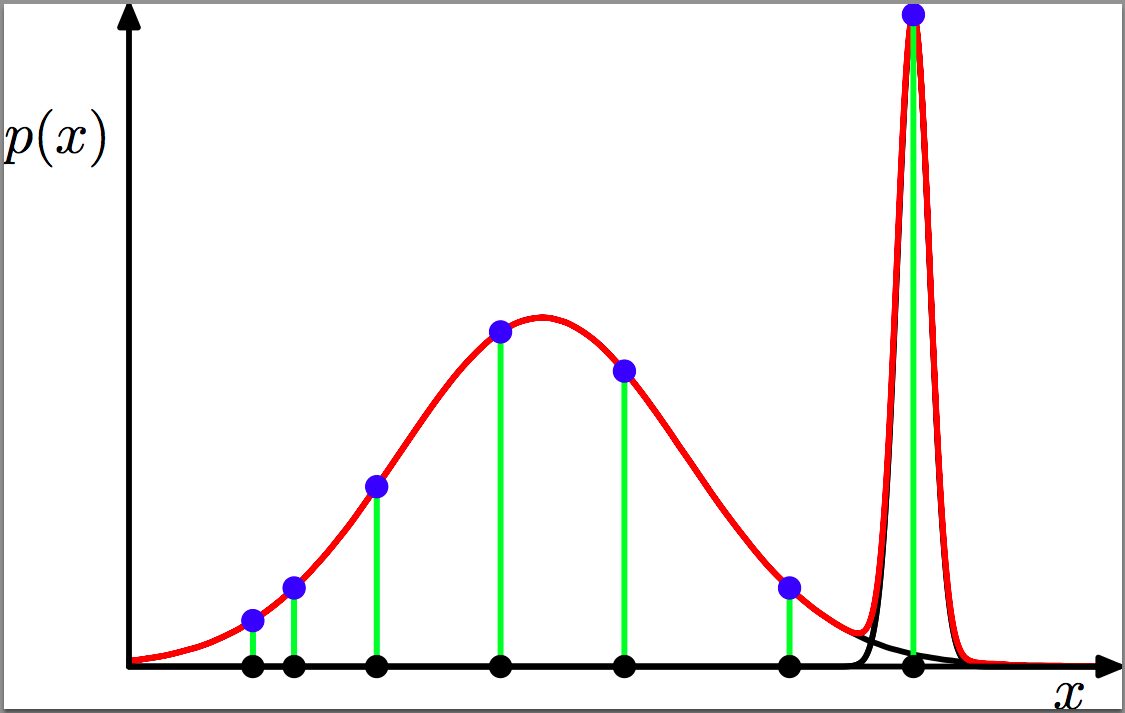
\includegraphics[height=0.4\textheight]{../Figures/clustering/gmm-singularity}
\par\end{center}


\begin{itemize}
\item Let $\sigma^{2}$ be the variance of the skinny component.
\item What happens to the likelihood as $\sigma^{2}\to0$?



\item In practice, we end up in local minima that do not have this problem.

\begin{itemize}
\item Or keep restarting optimization until we do.
\end{itemize}


\item Bayesian approach or regularization will also solve the problem.
\end{itemize}
\let\thefootnote\relax\footnotetext{\tiny{From Bishop's \emph{Pattern recognition and machine learning}, Figure 9.7.}}
\end{frame}

\begin{frame}{Gradient Descent / SGD for GMM}

\begin{itemize}
\item What about running gradient descent or SGD on
\begin{eqnarray*}
J(\pi,\mu,\Sigma) & = & -\sum_{i=1}^{n}\log\left\{ \sum_{z=1}^{k}\pi_{z}\cn\left(x_{i}\mid\mu_{z},\Sigma_{z}\right)\right\} ?
\end{eqnarray*}



\item Can be done \textendash{} but need to be clever about it.


\item Each matrix $\Sigma_{1},\ldots,\Sigma_{k}$ has to be positive semidefinite.


\item How to maintain that constraint?


\begin{itemize}
\item Rewrite $\Sigma_{i}=M_{i}M_{i}^{T}$, where $M_{i}$ is an unconstrained
matrix. 


\item Then $\Sigma_{i}$ is positive semidefinite. 

\end{itemize}
\end{itemize}
\end{frame}

\section{The EM Algorithm for GMM}
\begin{frame}{MLE for GMM}

\begin{itemize}
\item From the intro questions, we know that we can solve the MLE
  problem if the cluster assignments $z_i$ are known
  \begin{eqnarray*}
    n_z  & = & \sum_{i=1}^n \Ind(z_i=z)\\
    \hat{\pi}(z) & = & \frac{n_z}{n}\\
    \hat{\mu}_z & = & \frac{1}{n_z}\sum_{i:z_i=z} x_i\\
    \hat{\Sigma}_z & = & \frac{1}{n_z}\sum_{i:z_i=z} (x_i-\hat{\mu}_z)(x_i-\hat{\mu}_z)^T.
  \end{eqnarray*}
\item In the EM algorithm we will modify the equations to handle
  our evolving \textbf{soft assignments}, which we will call \textbf{responsibilities}.
\end{itemize}
\end{frame}

\begin{frame}{Cluster Responsibilities: Some New Notation}

\begin{itemize}
\item Denote the probability that observed value $x_{i}$ comes from cluster
$j$ by
\[
\gamma_{i}^{j}=\pr\left(Z=j\mid X=x_{i}\right).
\]



\item The \textbf{responsibility }that cluster $j$ takes for observation
$x_{i}$.



\item Computationally, 
\begin{eqnarray*}
\gamma_{i}^{j} & = & \pr\left(Z=j\mid X=x_{i}\right).\\
 & = & p\left(Z=j,X=x_{i}\right)/p(x)\\
 & = & \frac{\pi_{j}\cn\left(x_{i}\mid\mu_{j},\Sigma_{j}\right)}{\sum_{c=1}^{k}\pi_{c}\cn\left(x_{i}\mid\mu_{c},\Sigma_{c}\right)}
\end{eqnarray*}



\item The vector $\left(\gamma_{i}^{1},\ldots,\gamma_{i}^{k}\right)$ is
exactly the \textbf{soft assignment} for $x_{i}$.



\item Let $n_{c}=\sum_{i=1}^{n}\gamma_{i}^{c}$ be the ``number'' of points
``soft assigned'' to cluster $c$.
\end{itemize}
\end{frame}
\begin{frame}{EM Algorithm for GMM: Overview}
\begin{itemize}
  \item If we know $\pi$ and $\mu_j,\Sigma_j$ for all $j$ then we can
    easily find $\gamma_i^j=\pr(Z=j\mid X=x_i)$.
  \item If we know the (soft) assignments, we can easily find
    estimates for $\pi$, $\mu_j,\Sigma_j$ for all $j$.
  \item Repeatedly alternate the previous 2 steps.
\end{itemize}
\end{frame}
\begin{frame}{EM Algorithm for GMM: Overview}

\begin{enumerate}
\item Initialize parameters $\mu,\Sigma,\pi$.



\item ``E step''. Evaluate the responsibilities using current parameters:
\[
\gamma_{i}^{j}=\frac{\pi_{j}\cn\left(x_{i}\mid\mu_{j},\Sigma_{j}\right)}{\sum_{c=1}^{k}\pi_{c}\cn\left(x_{i}\mid\mu_{c},\Sigma_{c}\right)},\quad \text{for $i=1,\ldots,n$ and $j=1,\ldots,k$.}
\]




\item ``M step''. Re-estimate the parameters using responsibilities.
  [Compare with intro question.]
\begin{eqnarray*}
\mu_{c}^{\text{new}} & = & \frac{1}{n_{c}}\sum_{i=1}^{n}\gamma_{i}^{c}x_{i}\\
\Sigma_{c}^{\text{new}} & = & \frac{1}{n_{c}}\sum_{i=1}^{n}\gamma_{i}^{c}\left(x_{i}-\mu_{\text{MLE}}\right)\left(x_{i}-\mu_{\text{MLE}}\right)^{T}\\
\pi_{c}^{\text{new}} & = & \frac{n_{c}}{n},
\end{eqnarray*}
\item Repeat from Step 2, until log-likelihood converges. 
\end{enumerate}
\end{frame}

\begin{frame}{EM for GMM}

\begin{itemize}
\item Initialization
\end{itemize}
\begin{center}
\includegraphics[height=0.55\textheight]{../Figures/clustering/9\lyxdot 8a}
\par\end{center}

\let\thefootnote\relax\footnotetext{\tiny{From Bishop's \emph{Pattern recognition and machine learning}, Figure 9.8.}}

\end{frame}

\begin{frame}{EM for GMM}

\begin{itemize}
\item First soft assignment:
\end{itemize}
\begin{center}
\includegraphics[height=0.55\textheight]{../Figures/clustering/9\lyxdot 8b}
\par\end{center}

\let\thefootnote\relax\footnotetext{\tiny{From Bishop's \emph{Pattern recognition and machine learning}, Figure 9.8.}}

\end{frame}

\begin{frame}{EM for GMM}

\begin{itemize}
\item First soft assignment:
\end{itemize}
\begin{center}
\includegraphics[height=0.55\textheight]{../Figures/clustering/9\lyxdot 8c}
\par\end{center}

\let\thefootnote\relax\footnotetext{\tiny{From Bishop's \emph{Pattern recognition and machine learning}, Figure 9.8.}}

\end{frame}

\begin{frame}{EM for GMM}

\begin{itemize}
\item After 5 rounds of EM:
\end{itemize}
\begin{center}
\includegraphics[height=0.55\textheight]{../Figures/clustering/9\lyxdot 8e}
\par\end{center}

\let\thefootnote\relax\footnotetext{\tiny{From Bishop's \emph{Pattern recognition and machine learning}, Figure 9.8.}}

\end{frame}

\begin{frame}{EM for GMM}

\begin{itemize}
\item After 20 rounds of EM:
\end{itemize}
\begin{center}
\includegraphics[height=0.55\textheight]{../Figures/clustering/9\lyxdot 8f}
\par\end{center}

\let\thefootnote\relax\footnotetext{\tiny{From Bishop's \emph{Pattern recognition and machine learning}, Figure 9.8.}}

\end{frame}

\begin{frame}{Relation to $K$-Means}

\begin{itemize}
\item EM for GMM seems a little like $k$-means.



\item In fact, there is a precise correspondence.



\item First, fix each cluster covariance matrix to be $\sigma^{2}I$. 



\item As we take $\sigma^{2}\to0$, the update equations converge to doing
$k$-means.



\item If you do a quick experiment yourself, you'll find

\begin{itemize}
\item Soft assignments converge to hard assignments.
\item Has to do with the tail behavior (exponential decay) of
  Gaussian.
\end{itemize}
\item Can use $k$-means$++$ to initialize parameters of EM algorithm.
\end{itemize}
\end{frame}

\end{document}
